\documentclass[tikz, border=10pt]{standalone}
\usetikzlibrary{shapes, arrows.meta, positioning, calc}

\begin{document}
	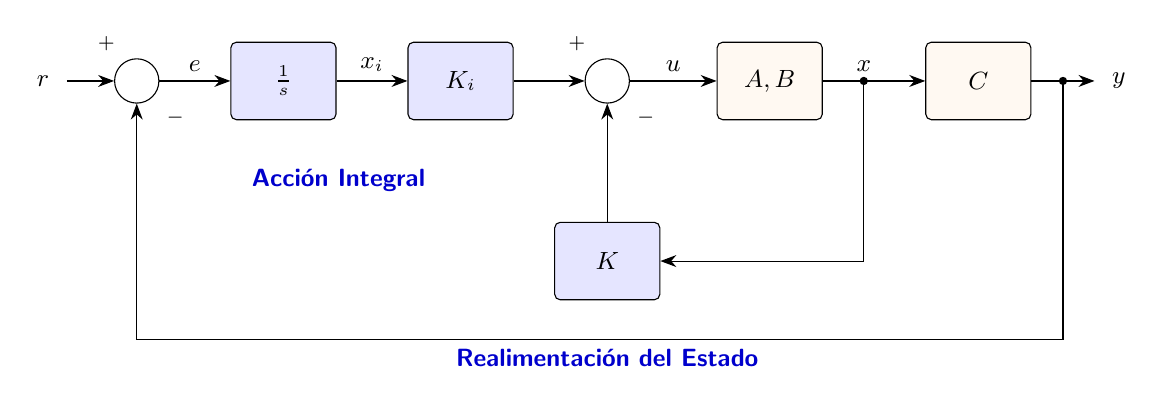
\begin{tikzpicture}[
		% Estilos de bloques coherentes con el lazo de control
		block/.style = {draw, fill=blue!10, rectangle, minimum height=2.8em, minimum width=3.8em, align=center, rounded corners=2pt, font=\small\sffamily},
		proc_block/.style = {draw, fill=orange!5, rectangle, minimum height=2.8em, minimum width=3.8em, align=center, rounded corners=2pt, font=\small\sffamily},
		sum/.style = {draw, circle, minimum size=16pt, inner sep=0pt, fill=white},
		input/.style = {coordinate},
		output/.style = {coordinate},
		node distance=1.2cm and 0.8cm,
		>={Stealth[scale=1.2]}
		]
		
		% --- EJE PRINCIPAL DE AVANCE (FORWARD PATH) ---
		\node [input] (r_in) {};
		\node [left=0.1cm of r_in, font=\small] {$r$};
		
		% Sumador de Error (Referencia - Salida)
		\node [sum, right=0.6cm of r_in] (sum_err) {};
		
		% Bloque Integrador (Genera el estado integral x_i)
		\node [block, right=0.9cm of sum_err] (int) {$\frac{1}{s}$};
		
		% Ganancia Integral K_i
		\node [block, right=0.9cm of int] (ki) {$K_i$};
		
		% Sumador de Control (Acción Integral - Realimentación de Estado)
		\node [sum, right=0.9cm of ki] (sum_u) {};
		
		% Planta (Matrices del sistema)
		\node [proc_block, right=1.1cm of sum_u] (plant) {$A, B$};
		\node [proc_block, right=1.3cm of plant] (c_mat) {$C$};
		
		% Salida del Sistema
		\node [output, right=0.8cm of c_mat] (salida) {};
		\node [right=0.1cm of salida, font=\small] {$y$};
		
		% --- RAMA DE REALIMENTACIÓN DE ESTADO ---
		\node [block, below=1.5cm of sum_u] (k_gain) {$K$};
		
		% --- CONEXIONES Y FLUJOS ---
		% Línea de entrada al error
		\draw [->] (r_in) -- (sum_err);
		\node [above left=0.05cm and -0.05cm of sum_err, font=\scriptsize] {$+$};
		
		% Lazo del error al integrador
		\draw [->] (sum_err) -- node[above, font=\small] {$e$} (int);
		
		% Del integrador a la ganancia Ki (Aquí nace el estado integral)
		\draw [->] (int) -- node[above, font=\small] {$x_i$} (ki);
		
		% De Ki al sumador de control
		\draw [->] (ki) -- (sum_u);
		\node [above left=0.05cm and -0.05cm of sum_u, font=\scriptsize] {$+$};
		
		% Del sumador de control a la planta
		\draw [->] (sum_u) -- node[above, font=\small] {$u$} (plant);
		
		% De la dinámica interna a la matriz de salida (Línea del estado x)
		\draw [->] (plant) -- node[above, pos=0.4, font=\small] {$x$} (c_mat);
		\draw [->] (c_mat) -- (salida);
		
		% --- LAZOS DE RETORNO (FEEDBACK LOOPS) ---
		% 1. Retorno del Vector de Estados (x) hacia la ganancia K
		\coordinate (branch_x) at ($(plant.east)!0.4!(c_mat.west)$);
		\fill (branch_x) circle (1.5pt);
		\draw [->] (branch_x) |- (k_gain.east);
		\draw [->] (k_gain.north) -- (sum_u.south);
		\node [below right=0.05cm and 0.05cm of sum_u, font=\scriptsize] {$-$};
		
		% 2. Retorno de la Salida Física (y) hacia el error (Lazo Externo)
		\coordinate (branch_y) at ($(c_mat.east)!0.5!(salida)$);
		\fill (branch_y) circle (1.5pt);
		\draw [->] (branch_y) |- ($(k_gain.south) - (0,0.5)$) -| (sum_err.south);
		\node [below right=0.05cm and 0.05cm of sum_err, font=\scriptsize] {$-$};
		
		% --- TEXTOS EXPLICATIVOS ---
		\node [below=0.5cm of int, xshift=0.7cm, font=\small\sffamily\bfseries, color=blue!80!black] {Acción Integral};
		\node [below=0.5cm of k_gain, font=\small\sffamily\bfseries, color=blue!80!black] {Realimentación del Estado};
		
	\end{tikzpicture}
\end{document}